% !TEX TS-program = pdflatex
% !TEX encoding = UTF-8 Unicode

% This file is a template using the "beamer" package to create slides for a talk or presentation
% - Talk at a conference/colloquium.
% - Talk length is about 20min.
% - Style is ornate.

% MODIFIED by Jonathan Kew, 2008-07-06
% The header comments and encoding in this file were modified for inclusion with TeXworks.
% The content is otherwise unchanged from the original distributed with the beamer package.

\documentclass[1pt]{beamer}
\usefonttheme[onlymath]{serif}
\usepackage{media9}
% \usepackage{beamerthemeshadow}
\usepackage[english]{babel}
% or whatever
\usepackage{caption}
\captionsetup[figure]{labelformat=empty}% redefines the caption setup of the figures environment in the beamer class.
\usepackage{lmodern}
\usepackage{units}
\usepackage[utf8]{inputenc}
\usepackage{amsmath}
% \usepackage{fullpage}
\usepackage{mathrsfs}
\usepackage{amsfonts}
\usepackage{amssymb}
\usepackage{fancyhdr}
\newcommand{\iu}{{i\mkern1mu}}
\newcommand{\bra}[1]{\langle #1 \vert}
\newcommand{\ket}[1]{\vert#1\rangle}
\newcommand{\avg}[1]{\left\langle#1\right\rangle}
\newcommand{\norm}[1]{\left\Vert #1 \right\Vert}
\newcommand{\braket}[2]{\left\langle #1 \vert#2 \right\rangle}
\newcommand{\obraket}[3]{\left\langle #1 \vert #2 \vert #3 \right \rangle}
\usepackage{times}
\usepackage[T1]{fontenc}
\newcommand{\dd}{\,\mathrm{d}}
\newcommand{\ddd}{\mathrm{d}}
\newcommand{\ii}{\mathrm{i}}
\usepackage{mhchem}
\usepackage{units}
% Copyright 2004 by Till Tantau <tantau@users.sourceforge.net>.
%
% In principle, this file can be redistributed and/or modified under
% the terms of the GNU Public License, version 2.
%
% However, this file is supposed to be a template to be modified
% for your own needs. For this reason, if you use this file as a
% template and not specifically distribute it as part of a another
% package/program, I grant the extra permission to freely copy and
% modify this file as you see fit and even to delete this copyright
% notice. 
\mode<presentation>
{
\usetheme{AnnArbor}
\usecolortheme{beaver}
\setbeamertemplate{frametitle}[default][center]
\setbeamertemplate{headline}{}
}

\usepackage{bm}


\title[Anderson localization ] % (optional, use only with long paper titles)
{An introduction to Anderson localization}

%\includegraphics[width=0.35\textwidth]{logo_fmf_uni-lj_en.pdf}\\[8ex] 

\author[Jan Šuntajs] % (optional, use only with lots of authors)
{Author: Jan Šuntajs \\ 
Mentor: prof. Janez Bonča \\
Comentor: doc. Lev Vidmar}
\centering
\titlegraphic{\includegraphics[width=4cm]{logo_fmf_uni-lj_en.pdf}
}

% - Give the names in the same order as the appear in the paper.
% - Use the \inst{?} command only if the authors have different
%   affiliation.

%\institute[University of Ljubljana, Faculty of Mathematics and Physics] % (optional, but mostly needed)
%{
%  \inst{1}%
%  Department of Computer Science\\
%  University of Somewhere
%  \and
%  \inst{2}%
%  Department of Theoretical Philosophy\\
%  University of Elsewhere}
% - Use the \inst command only if there are several affiliations.
% - Keep it simple, no one is interested in your street address.

%\date[CFP 2003] % (optional, should be abbreviation of conference name)
%{Conference on Fabulous Presentations, 2003}
% - Either use conference name or its abbreviation.
% - Not really informative to the audience, more for people (including
%   yourself) who are reading the slides online



% If you have a file called "university-logo-filename.xxx", where xxx
% is a graphic format that can be processed by latex or pdflatex,
% resp., then you can add a logo as follows:
%
% \pgfdeclareimage[height=0.8cm]{university-logo}{logo_fmf_uni-lj_en.pdf}
% \logo{\pgfuseimage{university-logo}}

% If you wish to uncover everything in a step-wise fashion, uncomment
% the following command: 

%\beamerdefaultoverlayspecification{<+->}


\begin{document}

\begin{frame}
  \titlepage
\end{frame}

% Structuring a talk is a difficult task and the following structure
% may not be suitable. Here are some rules that apply for this
% solution: 

% - Exactly two or three sections (other than the summary).
% - At *most* three subsections per section.
% - Talk about 30s to 2min per frame. So there should be between about
%   15 and 30 frames, all told.

% - A conference audience is likely to know very little of what you
%   are going to talk about. So *simplify*!
% - In a 20min talk, getting the main ideas across is hard
%   enough. Leave out details, even if it means being less precise than
%   you think necessary.
% - If you omit details that are vital to the proof/implementation,
%   just say so once. Everybody will be happy with that.

% \begin{frame}{Contents}

% \begin{enumerate}
% \item Introduction
% \vspace{10mm}
% \item Theoretical basics
% \vspace{10mm}
% \item Experiments
% \vspace{10mm}
% \item Conclusion
% \end{enumerate}


% \end{frame}


\begin{frame}{What is it about?}
\begin{minipage}[c]{0.9\textwidth}
\begin{itemize}
\item Conduction in \textbf{NON-INTERACTING} systems with \textbf{DISORDER}
\vspace{15mm}
\item Describes the role of \textbf{IMPURITIES}
\vspace{15mm}
\item Completely different than the \textbf{Drude} model:
$$ \sigma \propto l, \hspace{10mm} l: \text{the mean-free path}$$
\end{itemize}
\end{minipage}
\end{frame}

\begin{frame}{What does it predict?}
\centering{
\begin{itemize}
\item for some disorder: \hspace{5mm}
$ \sigma = 0$ \vspace{5mm}
\item seminal paper by \textbf{P. W. Anderson (1958)} \cite{Anderson}\vspace{5mm}
\item Nobel prize in \textbf{1977}
\end{itemize}}\vspace{2mm}
\begin{minipage}[c]{0.94\textwidth}
\begin{figure}
\centering{
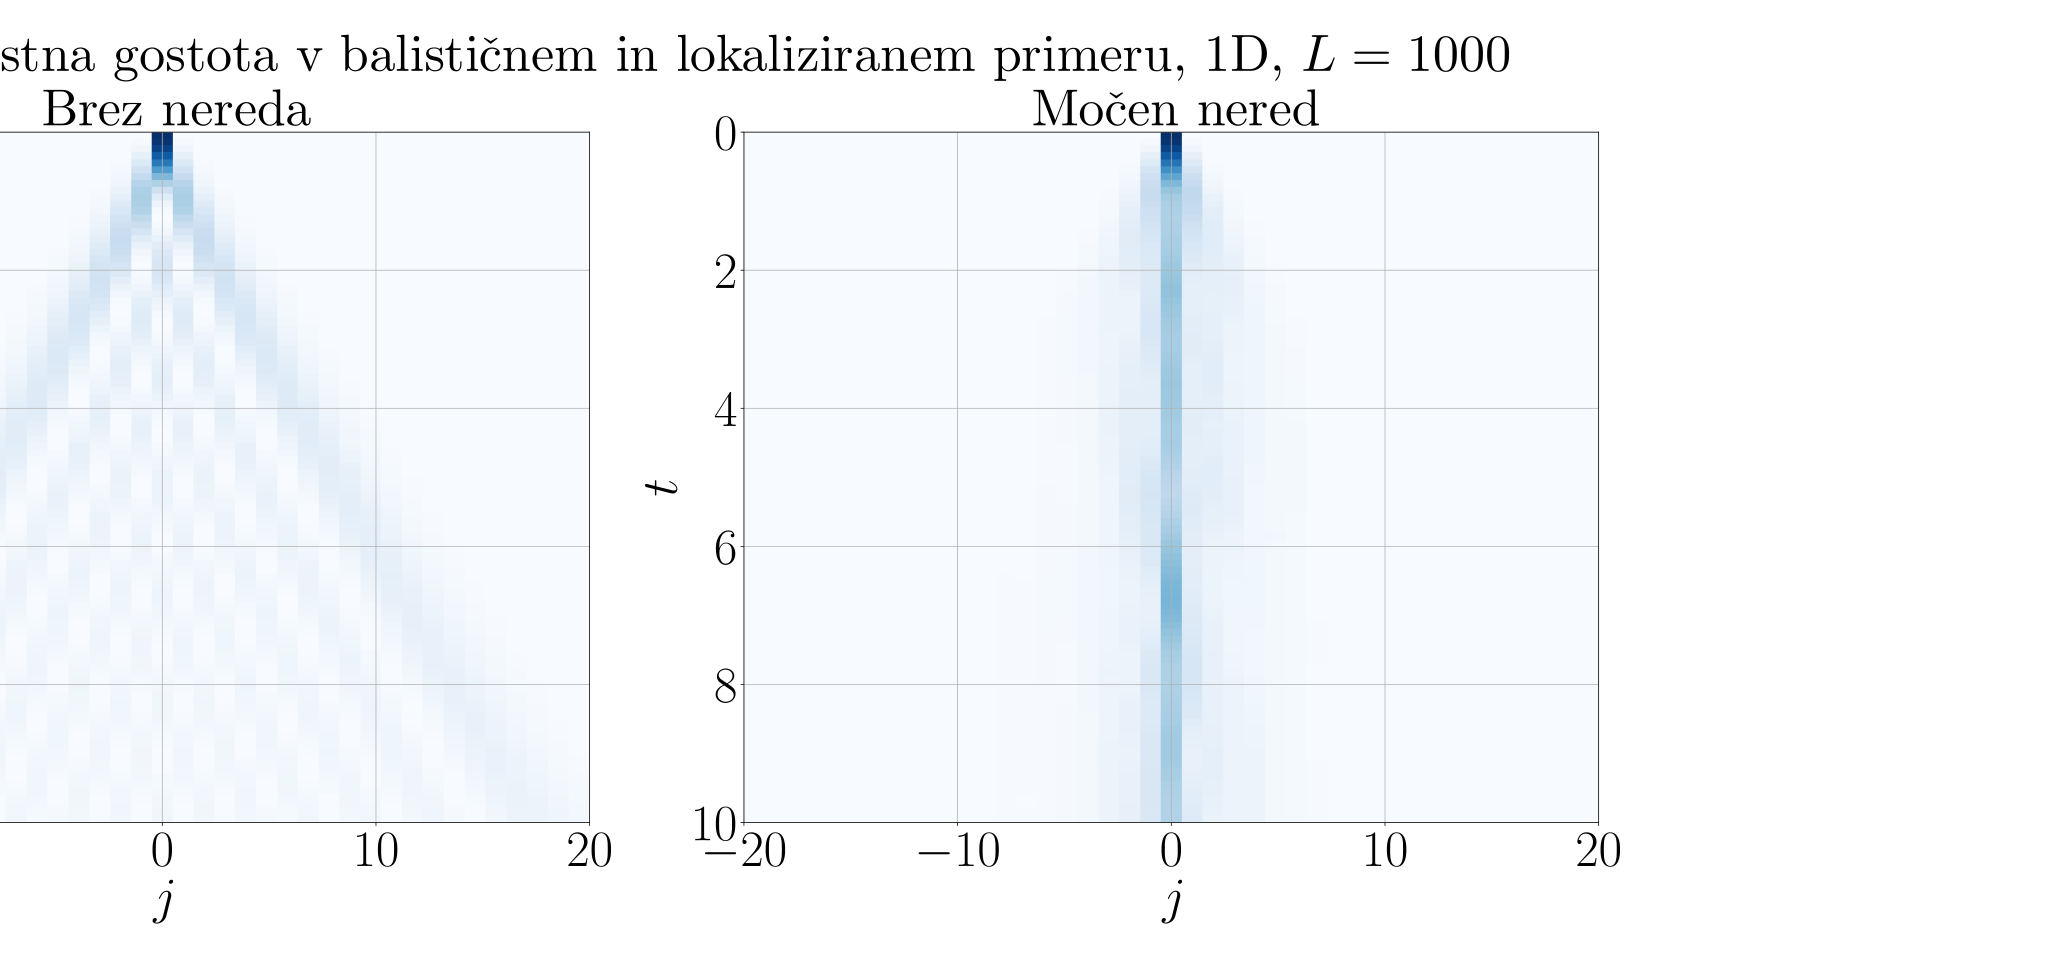
\includegraphics[width=1\textwidth]{1D_Anderson_localization_Seminar_scaling_analysis_D1_shape_1000_light_cone_double_presentation.pdf}}
% \caption{1D dynamics with no disorder and with strong disorder.}
\end{figure}
\end{minipage}
\end{frame}

\begin{frame}{Why does it (still) matter?}
What began in 1958 ...
\begin{figure}
\centering{
\includegraphics[width=0.9\textwidth]{and_orig_crop.pdf}}
% \caption{}
\end{figure} \pause
... still remains relevant today
\begin{figure}
\centering{
\includegraphics[width=0.8\textwidth]{huse_crop.pdf}}
% \caption{}
\end{figure}
\end{frame}

\begin{frame}{The current ``hot topic''}
\begin{itemize}
\item \textbf{Many-body localization (MBL)} - includes \textbf{INTERACTIONS}
\vspace{10mm}
\end{itemize}
\begin{minipage}[c]{0.6\textwidth}
Published in 2015:
\begin{figure}
\centering{
\includegraphics[width=1\textwidth]{mbl_crop.pdf}}
\caption{672 citations as of April 2018 acc. to Google Scholar.}
\end{figure}
\end{minipage}
\begin{minipage}[c]{0.38\textwidth}
\begin{itemize}
\vspace{5mm}
\item not our today's topic
\end{itemize}
\end{minipage}
\end{frame}

\begin{frame}{Outline}

\begin{enumerate}
\item The basic concepts of the Anderson localization
\vspace{10mm}
\item Models of disorder
\vspace{10mm}
\item Numerical simulations
\vspace{10mm}
\item Conclusion
\end{enumerate}


\end{frame}


% \begin{frame}{The model in a nutshell}
% % \begin{alertblock}{The model Hamiltonian}
% % \begin{equation*}\label{eq:ising_hamiltonian}
% % H_I=-J\sum\limits_i \hat{\sigma}_i^z\hat{\sigma}_{i+1}^z - h_{\perp}\sum\limits_i \hat{\sigma}_{i}^x.
% % \end{equation*}
% % \end{alertblock}{}

% % \begin{minipage}[c]{0.49\textwidth}
% % \begin{figure}
% % \centering{
% % \includegraphics[width=1\textwidth]{Sachdev_phase_diagram.pdf}}
% % \caption{The phase diagram.}
% % \end{figure}
% % \end{minipage}
% % \begin{minipage}[c]{0.4\textwidth}
% % \begin{figure}
% % \centering{
% % \includegraphics[width=1\textwidth]{zigzag_chain.jpg}}
% % \caption{The schematic of cobalt niobate}
% % \end{figure}
% % \end{minipage}\hfill

% \end{frame}

\begin{frame}{The basics}
\begin{minipage}[c]{0.5\textwidth}
\begin{itemize}
\item \textbf{DISORDER} $\rightarrow$ \textbf{(eigen)}states can localize
\vspace{10mm}
\item A localized state:
$$|\psi(\mathbf{r})| \sim \exp\left(|\mathbf{r} - \mathbf{r}_0 |/\xi \right)$$
\vspace{5mm}
\item explains \textbf{vanishing} transport
\vspace{10mm}
% \item An \textbf{interference} phenomenon.
\end{itemize}
\end{minipage}
\begin{minipage}[c]{0.4\textwidth}
\centering
Localization:
\begin{figure}
\centering{
\includegraphics[width=1\textwidth]{diff_loc_ext1_modified.pdf}}
% \caption{Extended and localized states.}
\end{figure}
\end{minipage}
\end{frame}

\begin{frame}{The important keynotes}
\begin{minipage}[c]{0.9\textwidth}
\begin{itemize}
\item An \textbf{interference} phenomenon
\vspace{12mm}		
\item Strong \textbf{dimensionality} dependence
\vspace{12mm}
\item Energy dependence $\rightarrow$ the \textbf{mobility edge}

% USE THIS LAST BULLET POINT TO INTRODUCE THE NEXT SLIDE
\end{itemize}
\end{minipage}
\end{frame}


% \begin{frame}{The enhanced back-scattering}
% % REFFER TO NANOPHYSICS HERE !!!! - to those who are attending it
% % and to those who did. If they didn't reffer to optics instead
% % do not forget RANDOMNESS - PHASES ARE RANDOM, SCATTERING is on
% % RANDOM POTENTIALS
% \begin{minipage}[c]{0.38\textwidth}
% \begin{itemize}
% \item calculation of the transition probability $w$
% \vspace{5mm}
% \item any two paths:
% $$w=|A_1 + A_2|^2=w_\mathrm{cl} + w_\mathrm{int}$$
% \vspace{5mm}
% \item time-reversed paths:
% $$w=4|A_1 |^2=2w_\mathrm{cl}$$
% % \item \textbf{QPT} at $h_{\perp_c}=J$
% \end{itemize}
% \end{minipage}\hfill
% \begin{minipage}[c]{0.5\textwidth}
% \begin{figure}
% \centering{
% \includegraphics[width=1\textwidth]{interference.jpg}}
% \caption{Path from $A$ to $B$ back to $A$ and its time-reverse}
% \end{figure}
% \end{minipage}
% \end{frame}
% BE VERBOSE HERE - MENTION EVERYTHING THAT HAS TO BE SAID, 
% COMMENT THE RESULT; WHAT IT MEANS; WHAT IT CAN DO in 1D and 2D

% \begin{frame}{Theoretical basics}
% % \begin{alertblock}{The model Hamiltonian}
% % \begin{equation*}\label{eq:ising_hamiltonian}
% % H_I=-J\sum\limits_i \hat{\sigma}_i^z\hat{\sigma}_{i+1}^z - h_{\perp}\sum\limits_i \hat{\sigma}_{i}^x.
% % \end{equation*}
% % \end{alertblock}{}

% % \begin{alertblock}{The Pauli matrices}
% % $$
% % \hat{\sigma}_i^z=\begin{pmatrix}
% % 1 & 0 \\ 0 & -1
% % \end{pmatrix}; \hspace{5mm}
% % \hat{\sigma}_i^x=\begin{pmatrix}
% % 0 & 1\\ 1 & 0
% % \end{pmatrix}; \hspace{5mm}
% % \hat{\sigma}_i^y=\begin{pmatrix}
% % 0 & -\iu \\ \iu & 0
% % \end{pmatrix}
% % $$
% % \end{alertblock}{}
% % \begin{alertblock}{The $\hat{\sigma}_i^x$ operator eigenstates}
% % \begin{equation*}
% % \begin{split}
% % \ket{\rightarrow}_i& = \left(\ket{\uparrow}_i + \ket{\downarrow}_i\right)/\sqrt{2}, \\
% % \ket{\leftarrow}_i& = \left(\ket{\uparrow}_i - \ket{\downarrow}_i\right)/\sqrt{2}.
% % \end{split}
% % \end{equation*}
% % \end{alertblock}{}
% \end{frame}

% SAY THAT EBS CAN GIVE AN INTUITIVE EXPLANATION BUT IS 
% INSUFFICIENT IN ACCOUNTING FOR THE COMPLEX DIMENSIONALITY DEPENDENCE
% NOTE THAT THE COMPLETE TREATMENT IS STILL MISSING - WE RESORT TO 
% PHENOMENOLOGICAL THEORIES SUCH AS THE SCALING THEORY
\begin{frame}{The scaling theory  }
\begin{itemize}
\item scaling of the \textbf{conductance} $g$ of 
a \textbf{hypercube} $L^d$ \vspace{3mm} \cite{scaling}
\end{itemize}
\begin{minipage}[c]{0.38\textwidth}
\begin{itemize}
% \vspace{15mm}
\item \textbf{Ohmic} conductor:
$$g=\sigma L^{d-2}$$
\vspace{5mm}
\item \textbf{Localized} regime:
$$g\propto \exp(-L)$$
% \item \textbf{QPT} at $h_{\perp_c}=J$
\end{itemize}
\end{minipage}\hfill
\begin{minipage}[c]{0.6\textwidth}
\begin{figure}
\centering{
\includegraphics[width=1\textwidth]{beta_diagram.jpg}}
\caption{Transition between ext. and loc. states is only possible in 3D. Taken from \cite{50yearsof}.}
\end{figure}
\end{minipage}
\end{frame}
\begin{frame}{The scaling theory}
\begin{minipage}[c]{0.36\textwidth}
\begin{alertblock}{\centering\textbf{1D, 2D}}
\centering localization for any finite disorder
\end{alertblock}\vspace{0.65cm}
\begin{alertblock}{\centering\textbf{3D}}
\centering localization for some critical disorder
\end{alertblock}\vspace{0.35cm}
\end{minipage}\hfill
\begin{minipage}[c]{0.6\textwidth}
\vspace{5mm}
\begin{figure}
\centering{
\includegraphics[width=1\textwidth]{beta_diagram.jpg}}
\caption{Transition between ext. and loc. states is only possible in 3D. Taken from \cite{50yearsof}.}
\end{figure}
\end{minipage}
\end{frame}

\begin{frame}{The mobility edge}

\begin{figure}
\centering{
\includegraphics[width=1\textwidth]{mob_edge_schematic.pdf}}
%\caption{Single-excitation dispersion relation}
\end{figure}


\end{frame}

\begin{frame}{The models of disorder}
\begin{minipage}[c]{0.57\textwidth}
\begin{itemize}
\item somehow distorting the \textbf{ideal crystal}\vspace{8mm}  
\end{itemize}
\begin{alertblock}{\centering\textbf{A generic Hamiltonian}}
$$
H=\frac{\hat{p}^2}{2m} + \sum\limits_{j=1}^N V_j(\mathbf{r}-\mathbf{R}_j)
$$
\end{alertblock}\vspace{10mm}
\begin{itemize}
\item we consider the \textbf{Anderson model}
\end{itemize}
\end{minipage}\hfill
\begin{minipage}[c]{0.4\textwidth}
\begin{figure}
\centering{
\includegraphics[width=1\textwidth]{disorder_scheme.pdf}}
\caption{Ideal crystal, compositional, structural and kinetic disorder. Adapted acc. to \cite{Kramer}.}
\end{figure}
\end{minipage}
\end{frame}

\begin{frame}{Our model - the \textbf{Anderson model}}
\begin{alertblock}{The Anderson Hamiltonian \cite{Anderson}}
\begin{equation*}\label{eq:ising_hamiltonian}
H=\sum\limits_j \varepsilon_j c^\dagger_jc_j - V\sum\limits_{\text{n.n.}} c^\dagger_{i}c_j + \text{h.c.}
\end{equation*}
\end{alertblock}{}
\begin{minipage}[c]{0.48\textwidth}
\begin{alertblock}{Probability distribution of $\varepsilon_j$}
\begin{equation*}\label{eq:ising_hamiltonian}
p(\varepsilon_j)=\frac{1}{2W}\Theta(W-|\varepsilon_j|)
\end{equation*}
\end{alertblock}{}
\begin{figure}
\centering{
\includegraphics[width=1\textwidth]{prob_dist.pdf}}
% \caption{The model in 2D.}
\end{figure}
\end{minipage}\hfill
\begin{minipage}[c]{0.45\textwidth}
\begin{figure}
\centering{
\includegraphics[width=1\textwidth]{hopping_picture_50years.jpg}}
\caption{The model in 2D. Taken from \cite{50yearsof}.}
\end{figure}
\end{minipage}\hfill
\end{frame}
\begin{frame}{The Anderson model}

% \begin{minipage}{0.38\textwidth}
% \begin{figure}
% \centering{
% \includegraphics[width=1\textwidth]{bands.png}}
% %\caption{Single-excitation dispersion relation}
% \end{figure}
% \end{minipage}\hfill\vspace{5mm}
% \begin{minipage}{0.6\textwidth}
% \begin{itemize}
% 	\item Two mobility edges in 3D
% \end{itemize}
% \end{minipage}\\
% \begin{minipage}{0.38\textwidth}
% % Two mobility edges in 3D
% \end{minipage}\hfill\vspace{5mm}
% \begin{minipage}{0.7\textwidth}
% \begin{figure}
% \centering{
% \includegraphics[width=1\textwidth]{mobility_edge_DOS.pdf}}
% %\caption{The continuum splits into discrete states.}
% \end{figure}
% \end{minipage}

\begin{itemize}
	\centering \item Two mobility edges in 3D
\end{itemize}
\begin{figure}
\centering{
\includegraphics[width=1\textwidth]{mobility_edge_DOS_modified.pdf}}
%\caption{The continuum splits into discrete states.}
\end{figure}
\end{frame}

\begin{frame}{My work - the numerical simulations}
\begin{itemize}
\item How to extract features of the Anderson localization numerically?\vspace{5mm}
 \begin{itemize}
	\item implementation in 1D, 2D and 3D \vspace{2mm}
	\item calculations were run at the F-1 cluster at IJS \vspace{2mm}
	\item Full diagonalization and time evolution calculations
\end{itemize}\vspace{5mm}
\item Two localization criteria: \vspace{5mm}
\begin{itemize}
	\item the \textbf{inverse participation ratio} (IPR)\vspace{2mm}
	\item the \textbf{absence of diffusion}
\end{itemize}
\end{itemize}
\end{frame}

\begin{frame}{Localization criteria - the IPR}
\begin{alertblock}{The definition}
\begin{equation*}
P^{-1}=\sum\limits_\mathbf{r} |\psi(\textbf{r})|^4, \hspace{5mm} \norm{\psi}=1.
\end{equation*}
\end{alertblock}{}\vspace{5mm}
\begin{itemize}
	\item sum over the lattice sites
	\end{itemize}\vspace{5mm}
\begin{alertblock}{\centering{If $L$ large enough}}
$$
P^{-1} \propto\begin{cases}
&1/L^d, \hspace{5mm} \text{extended} \\
&\text{const}, \hspace{5mm} \text{localized} 
\end{cases}
$$ 
% smaller for extended states, larger for extended ones \vspace{10mm}
% \item Full Hamiltonian diagonalization needed 
\end{alertblock}{}
% \begin{figure}
% \centering{
% \includegraphics[width=1\textwidth]{1D_Anderson_localization_Seminar_scaling_analysis_D1_shape_1000_ipr_plots.pdf}}
% %\caption{The continuum splits into discrete states.}
% \end{figure}
\end{frame}

\begin{frame}{IPR - the results}
\begin{figure}
\centering{
\includegraphics[width=0.75\textwidth]{1D_Anderson_localization_Seminar_scaling_analysis_D1_shape_1000_ipr_plots_presentation.pdf}}
%\caption{The continuum splits into discrete states.}
\end{figure}
\begin{figure}
\centering{
\includegraphics[width=0.75\textwidth]{2D_Anderson_localization_Seminar_scaling_analysis_D2_shape_100_100_ipr_plots_presentation.pdf}}
%\caption{The continuum splits into discrete states.}
\end{figure}
\end{frame}

\begin{frame}{IPR 3D}
\begin{figure}
\centering{
\includegraphics[width=0.9\textwidth]{3D_Anderson_localization_Seminar_scaling_analysis_D3_shape_22_22_22_eigensys_plots_single_presentation_nozero.pdf}}
%\caption{The continuum splits into discrete states.}
\end{figure}
\end{frame}

\begin{frame}{Absence of diffusion}
\begin{alertblock}{Time evolution}
\begin{equation*}
\ket{\psi, t+\mathrm{d}t}=\exp\left(-\mathrm{i}\hat{H}\dd t\right)\ket{\psi, t},
\end{equation*}
\end{alertblock}{}\vspace{2mm}
\begin{minipage}{0.28\textwidth}
\begin{alertblock}{}
$$
\hat{R^2}=\sum\limits_{\mathbf{r}_j} \mathbf{r}_j^2 \hat{n}_{\mathbf{r}_j}, 
$$
\end{alertblock}{}
\begin{alertblock}{}
$$
\beta(t)=\frac{\dd \log R}{\dd \log t}
$$
\end{alertblock}{}
\end{minipage}\hfill
 \begin{minipage}{0.7\textwidth}
\begin{figure}
\centering{
\includegraphics[width=1\textwidth]{1D_Anderson_localization_Seminar_scaling_analysis_D1_shape_2000_r_sq_dynamics_presentation.pdf}}
%\caption{Single-excitation dispersion relation}
\end{figure}
\end{minipage}
\begin{alertblock}{}
$$
R(t)=\sqrt{\bra{\psi,t} \hat{R^2}\ket{\psi,t}-\bra{\psi,0} \hat{R^2}\ket{\psi,0}} 
$$
\end{alertblock}{}
\end{frame}

\begin{frame}{Absence of diffusion, 2D}
\begin{figure}
\centering{
\includegraphics[width=1\textwidth]{2D_Anderson_localization_Seminar_scaling_analysis_D2_shape_500_500_r_sq_dynamics_presentation.pdf}}
%\caption{Single-excitation dispersion relation}
\end{figure}

\end{frame}
\begin{frame}{Conclusion}
\begin{itemize}
	\item A first step towards the description of conduction in real systems. \vspace{10mm}
	\item A nontrivial numerical implementation.\vspace{10mm}
	\item Needed in understanding the MBL phenomena, the current ``hot topic.''
\end{itemize}
\end{frame}
\begin{frame}{References and sources of images}
   
 \begin{thebibliography}{10}
   
 \beamertemplatebookbibitems
 % Start with overview books.



   
 \beamertemplatearticlebibitems
 % Followed by interesting articles. Keep the list short. 

\bibitem{Anderson}
Anderson, P. (1958). \emph{Absence of Diffusion in Certain Random Lattices.} Physical Review, \textbf{109}(5), pp.1492-1505.
\bibitem{scaling}
Abrahams E., Anderson P. W., Licciardello, D. and Ramakrishnan, T.V. (1979).\emph{Scaling Theory of Localization: Absence of Quantum Diffusion in Two Dimensions.} Phys. Rev. Lett. \textbf{42}(10), 673
\bibitem{Kramer}
Kramer, B. and MacKinnon, A. (1993). \emph{Localization: theory and experiment.} Reports on Progress in Physics, \textbf{56}(12), pp.1469-1564.
\bibitem{50yearsof}
Lagendijk, A., Tiggelen, B. and Wiersma, D. (2009). \emph{Fifty years of Anderson localization.} Physics Today, \textbf{62}(8), pp.24-29.



 \end{thebibliography}
\end{frame}

\end{document}


